\documentclass{mcmthesis}
\mcmsetup{CTeX = false,   % 使用 CTeX 套装时,设置为 true
        tcn =2008722, problem = A,
        sheet = true, titleinsheet = false, keywordsinsheet = true,
        titlepage = false, abstract = true}
\usepackage{newtxtext}%\usepackage{palatino}

\usepackage{url}
\usepackage{threeparttable}
\usepackage{chngpage}
\usepackage{array}
\usepackage{booktabs}
\usepackage{longtable}

\usepackage{epstopdf}
\usepackage{float}
\usepackage{subfig}
\usepackage{amsmath}
\usepackage{cases}


\newcommand{\upcite}[1]{\textsuperscript{\textsuperscript{\cite{#1}}}}
\usepackage[numbers,sort&compress]{natbib}
%%% 实现参考文献标号在右上角
\usepackage{geometry}
\geometry{left=1.3in,right=1.3in,bottom=1.25in}
\usepackage{lipsum}
\title{The \LaTeX{} Template for MCM Version \MCMversion}
\author{\small \href{http://www.latexstudio.net/}
  {
\includegraphics[width=7cm]{mcmthesis-logo}}}
\date{\today}
\usepackage{verbatim}
\begin{document}
\begin{abstract}
	This is the age of information explosion. Numbers, text, video and audio are all information. How to dig out the instructive information we are interested in from the large amount of data is crucial. A rating model based on user comments is constructed.
	
	To understand consumer preferences and basic information, we used TextBlob, a natural language processing library in Python, to perform word frequency statistics and sentiment analysis on the content of product reviews. We have seen an exponential increase in the number of reviews, with more and more consumers choosing to shop online, with beauty and baby products more popular. Specific quality descriptors of text-based reviews such as' love ', 'disappointed', and others, strongly associated with rating levels.
	
	In order to understand product reputation and predict the success of product promotion, we defined product reputation score and product future development score through a rating model based on user reviews. In order to understand whether the product evaluation content has the Matthew effect, we use the moving average algorithm in the time series to analyze the correlation between the number of comments of each product evaluation quantity and the number of comments, and find that the comments of the following commenters are correlated with the comments of the previous commenters.
	
	Finally, we performed sensitivity analysis and extended the model.
\begin{keywords}
keyword1; keyword2
\end{keywords}
\end{abstract}
\maketitle
%% Generate the Table of Contents, if it's needed.
\thispagestyle{empty}
\tableofcontents

%\newpage
%\thispagestyle{empty}
%\title{fish of scotland}
%\lipsum{5}

%%
%Generate the Memorandum, if it's needed.
%\memoto{\LaTeX{}studio}
%\memofrom{Liam Huang}
%\memosubject{Happy \TeX{}ing!}
%\memodate{\today}
% \logo{\LARGE I'm pretending to be a LOGO!}
%\begin{memo}[Memorandum]
%	\lipsum[1-3]
%\end{memo}

\newpage
\setcounter{page}{1}
%%

\section{Introduction}
\subsection{Background}

.
\subsection{Restatement of the Problem}%{问题重述}


\subsection{Overview of Our Work}%{我们做的工作概览}




\section{Assumptions and Justifications}
\begin{itemize}
\item
\item
\item
\item
\end{itemize}


\section{Notation}%{符号说明}
\begin{center}
	%\begin{longtable}{m{.1\textwidth}m{.8\textwidth}m{.4\textwidth}}
	\begin{longtable}{cl}
		\caption{    }\\ %名字
		\hline
		Symbol& Description  \\
		\hline
		$   $   &
		\\
		$   $   &
		\\
		$   $   &
		\\
		$   $   &
		\\
		$   $   &
		\\
		$   $   &
		\\
		$   $   &
		\\
		$   $   &
		\\
		$   $   &
		\\
		$   $   &
		\\
		
	\end{longtable}
\end{center}


\section{Name of Model}



\section{Name of Mode2}




\section{ Results and Recommendations}
\subsection{Inform Online Sales Strategy}
First, we do some basic analysis of the known raw data to understand the basic situation of online sales. Then we raised a series of questions that the sun company might be interested in.

1. Is online shopping becoming more common in America?

2. Will online sales replace traditional marketing?

3. Whose user experience is better online than traditional sales?

4. What products are suitable for online sales?

\begin{figure}[H]
	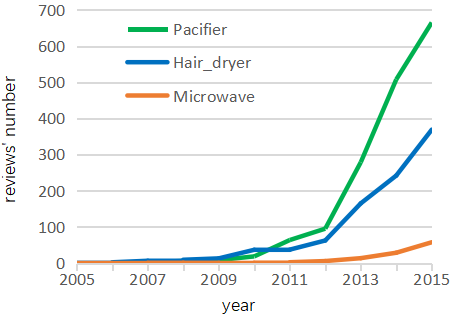
\includegraphics[width=7cm]{./figures/q1p1.png}
	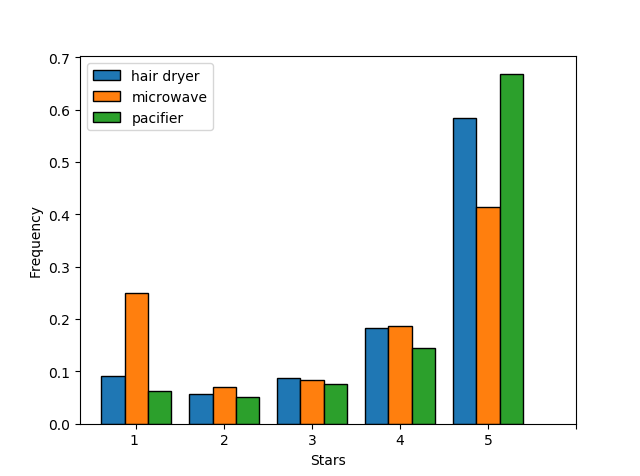
\includegraphics[width=7cm]{./figures/z1.png}
	\caption{Figure on the Left: the average number of monthly reviews of the three products per year; Figure on the right: star frequency of all data of three types of product} \label{z1_q1p1}
\end{figure}

We know that the number of comments is directly proportional to the number of online shoppers, so we can see the figure on the right as the relationship between the number of online shoppers and time. From the left chart, we can find that before 2008, very few people chose to shop online. After 2008, online shopping became more and more popular. To analyze the reasons, the subprime mortgage crisis in the United States in 2008 triggered the global financial crisis, which led to the failure of many banks and the collapse of small and medium-sized enterprises. In order to survive, many small businesses have switched to online sales, because it is known that online sales cost is small, with no rent, sales staff.

We found that the number of online shoppers increased exponentially after 2008, indicating that online shopping is becoming more and more popular with customers. We have reasons to believe that online sales will beat traditional marketing, and online shopping will become the new shopping habit of people in the new era. Here we strongly suggest the sun company to develop an online sales business.

Pacifiers are baby products, hairdryers are beauty products, and microwave ovens are large appliances. On the left, we found that compared to hairdryers and pacifiers, the number of microwave reviews is very small, that is, the number of people who buy microwave ovens online is very small. Combined with the picture on the right, the one-star microwave oven can be found to be very large, which indicates that consumers do not like to buy large appliances online. In summary, beauty and baby products are more suitable for online sales.

The figure on the right shows the star distribution map of online reviews of three kinds of products. The frequency of five-star pacifiers and hairdryer is more than 50\%, which indicates that most people have a good online shopping experience for these products. Everyone can buy things that are both cheap and easy to use to meet their needs.

Through the NLTK of Python, the TF-IDF algorithm is used to calculate the word frequency of comments, and the word cloud graph is drawn as follows through a word cloud.

\begin{figure}[H]
	\centering
	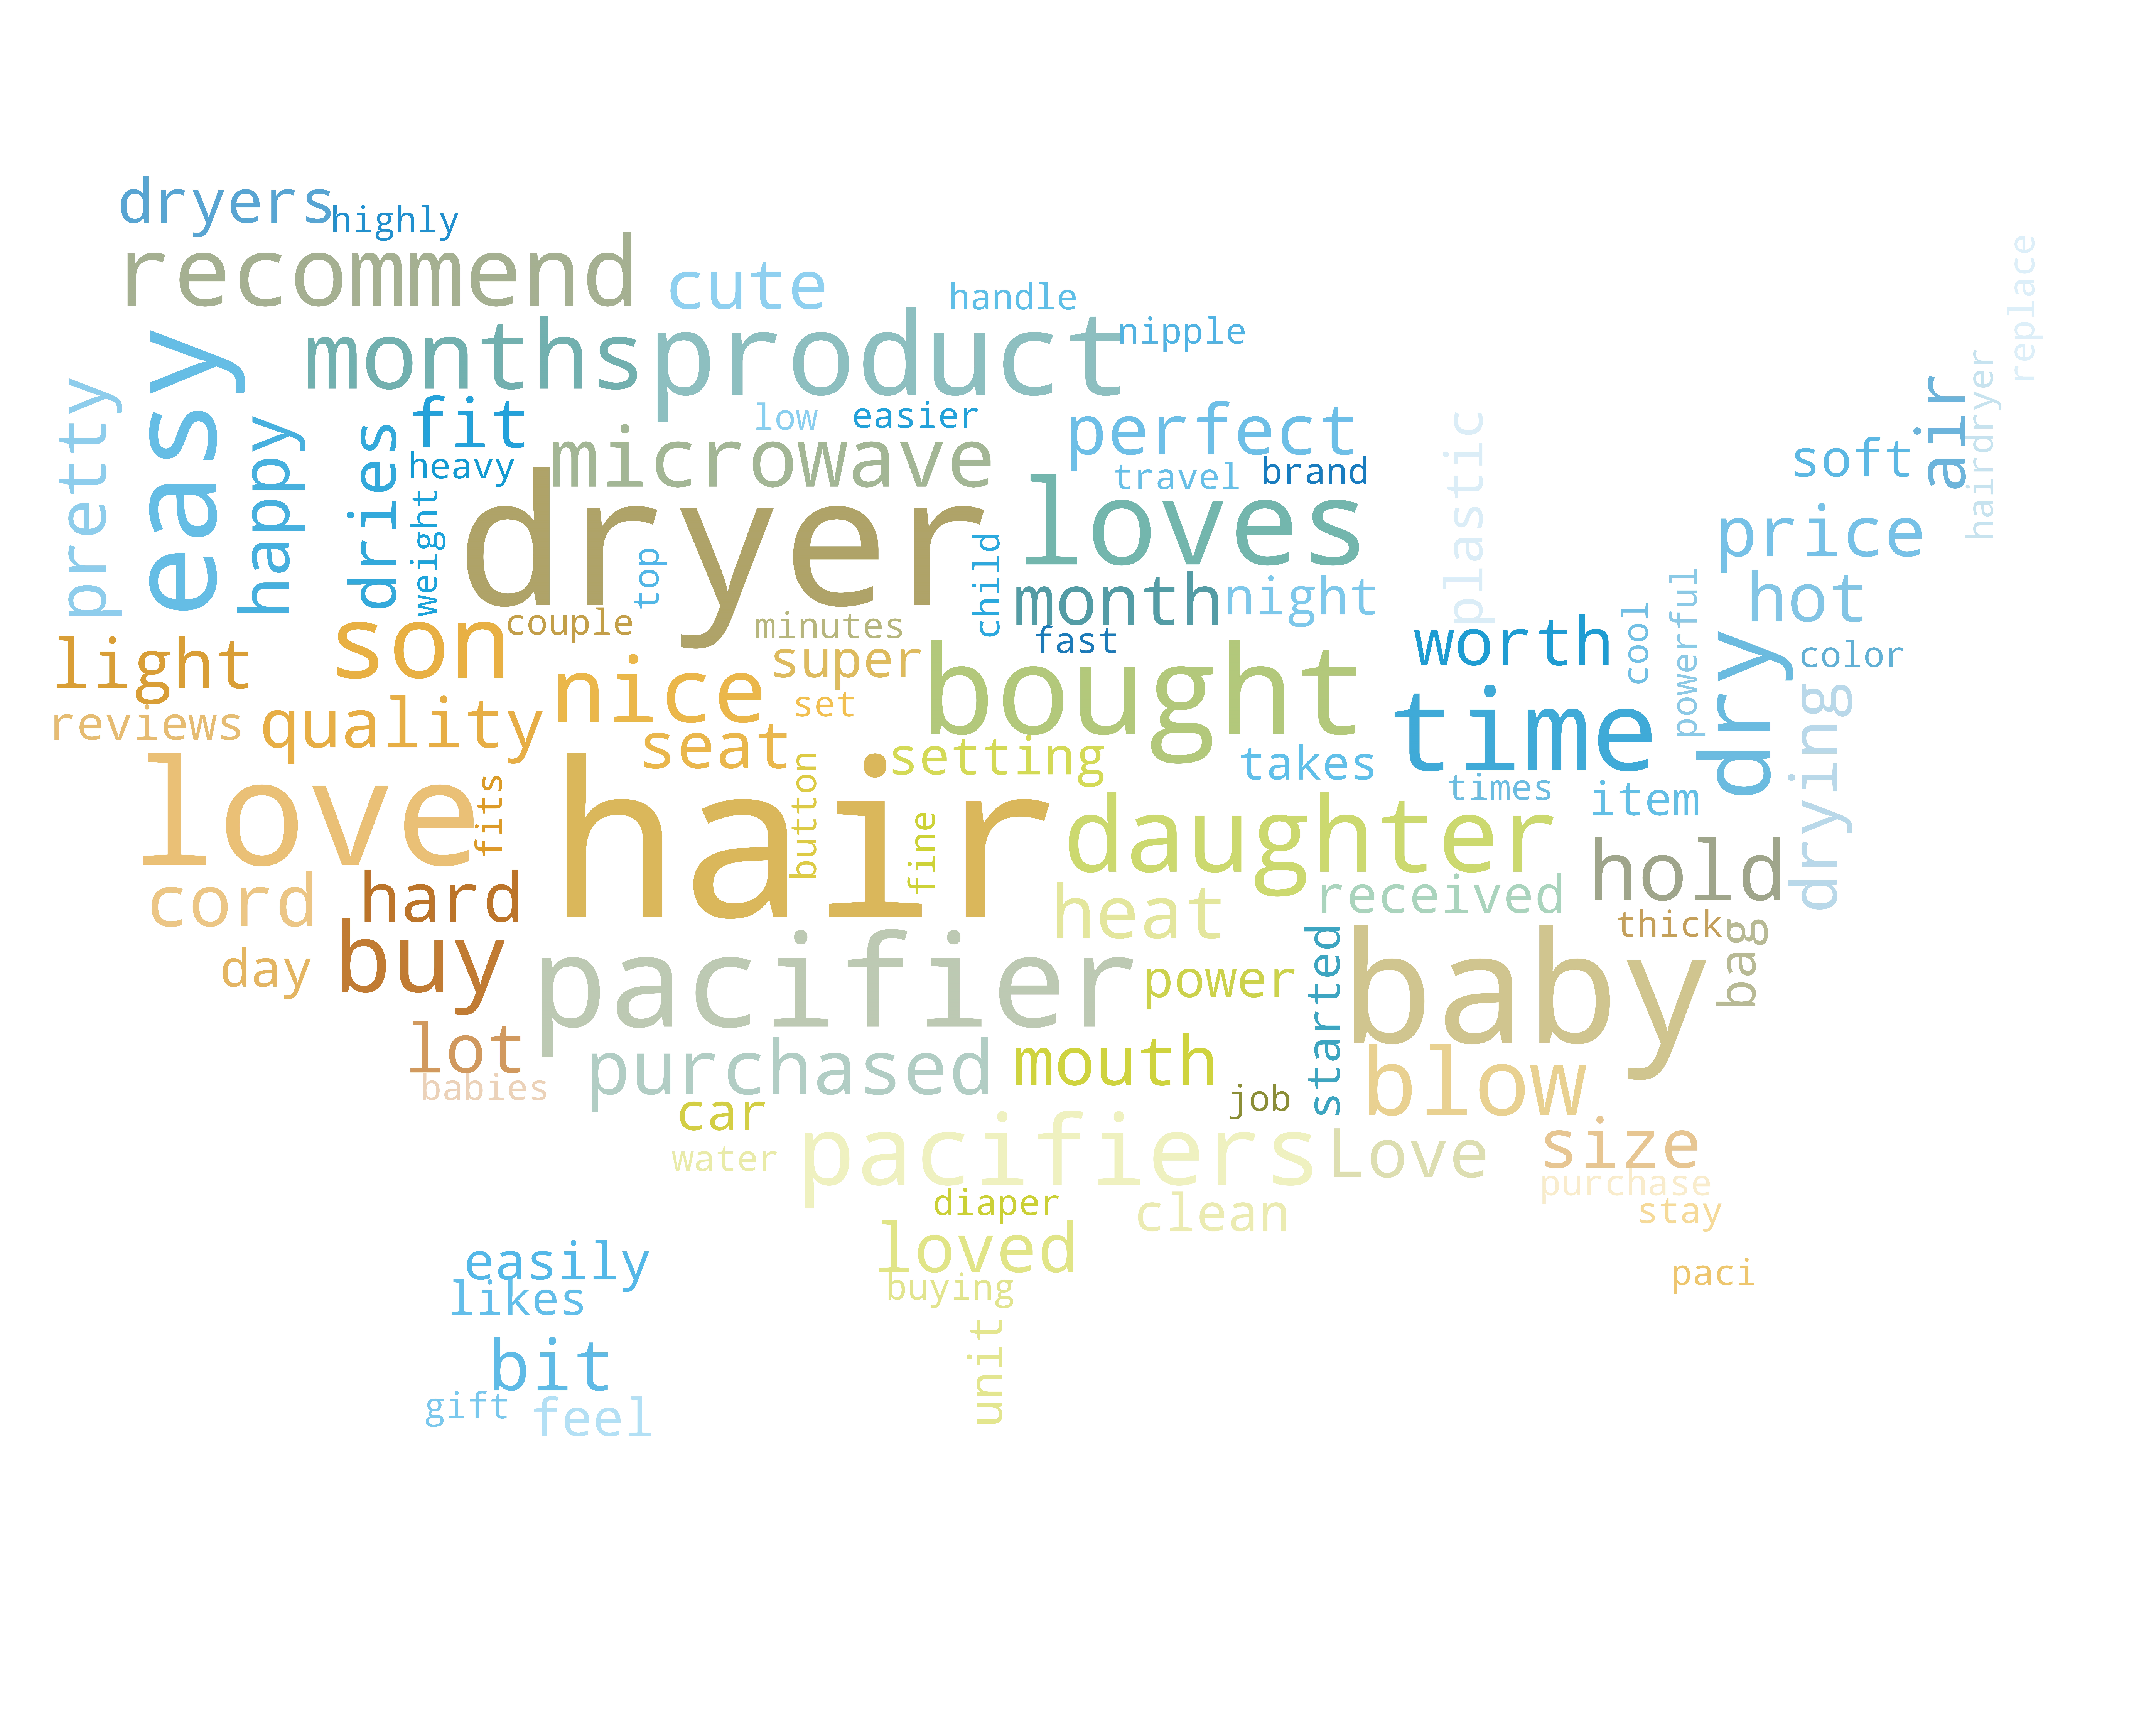
\includegraphics[width=10cm]{./figures/wc.png}
	\caption{The word cloud map of all comments in three data sets} \label{wordCloud}
\end{figure}

According to the figure \ref{wordCloud}, consumers are most concerned about the quality and price of products. When products are launched on the online market, both the quality of the products and the "beautiful" price should be guaranteed.

\subsection{Potentially Important Design Features}

In the study of consumer reviews, we use the word frequency algorithm to get the high-frequency words corresponding to the stars of each product. We can find that quality, service, and price are the most important concerns for consumers. Now we want to understand the potentially important design features of specific products to enhance product satisfaction. Due to the space limitation, we will only give the frequency table of baby pacifier words.

\begin{figure}[H]
	\centering
	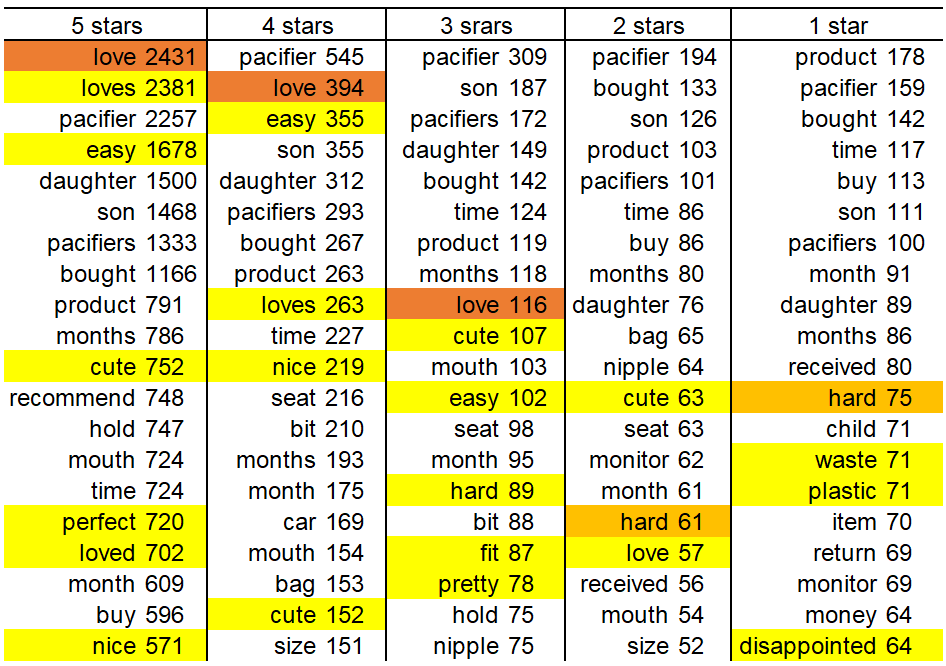
\includegraphics[width=14cm]{./figures/pdc2.png}
	\caption{Top20:The frequency of words corresponding to different stars of the baby pacifier} \label{pdc1}
\end{figure}

Bad reviews are what we're really focused on, where we can identify areas where consumers are dissatisfied,so we adjust our product or online sales strategy to improve our competitiveness. As can be seen from the figure \ref{pdc1} :

1. When evaluating products, consumers prefer to describe their subjective feelings rather than product attributes.

2. Specific quality descriptors of text-based reviews such as' love ', 'disagree', and others, strongly associated with rating levels.

3. In the low-star rating, "hard" and "plastic" reflect that the potentially important design functions of the baby nipple are its hardness and material safety; Potentially important design functions of the hairdryer are drying effect and service life. Potentially important design features of microwave ovens are functional diversity and after-sales service.

\subsection{The Product’s Reputation}

Consumers' real evaluation score only considers the content and stars of the review, not the importance of the review. The four most important factors when considering product reputation are star rating, reviews, vine, and helpful votes. \upcite{WannThe}

Each commenter contributes $p_{I}$to the product's reputation:

\begin{equation}\label{q2}
p_{i}=\sum_{i}^{n_i}[s_{i}+k_{i}(r_{i1}+r_{i2})]
\end{equation}

The reputation of a product takes into account the reputation of the product rated by each reviewer at a certain point in time, and the following indicators are obtained. This indicator can describe the reputation of the product in a certain period, whether it goes down or up, where $n_k$ is the number of reviews of j product in the k month. K month reputation score of j product $rp_{jk}$:

\begin{equation}\label{gs1}
rp_{jk}=\frac{\sum_{i}^{n_k}[s_{ji}+k_{ji}(r_{ji1}+r_{ji2})]}{n_i}
\end{equation}

In drawing the presentation, we did some manipulation on the data: each reviewer's reputation for the product was divided into $rp_{I}$by converting it to a number on $[-1,1]$. The value on $(0,1]$indicates that each reviewer's contribution to the product's reputation is positive; The value on $[-1,0)$indicates that each reviewer has a negative reputation contribution to the product; 0 indicates that each reviewer has no reputation contribution to the product; since the maximum number of baby pacifiers is 18,939, the data we selected is pacifier data.

\begin{figure}[H]
	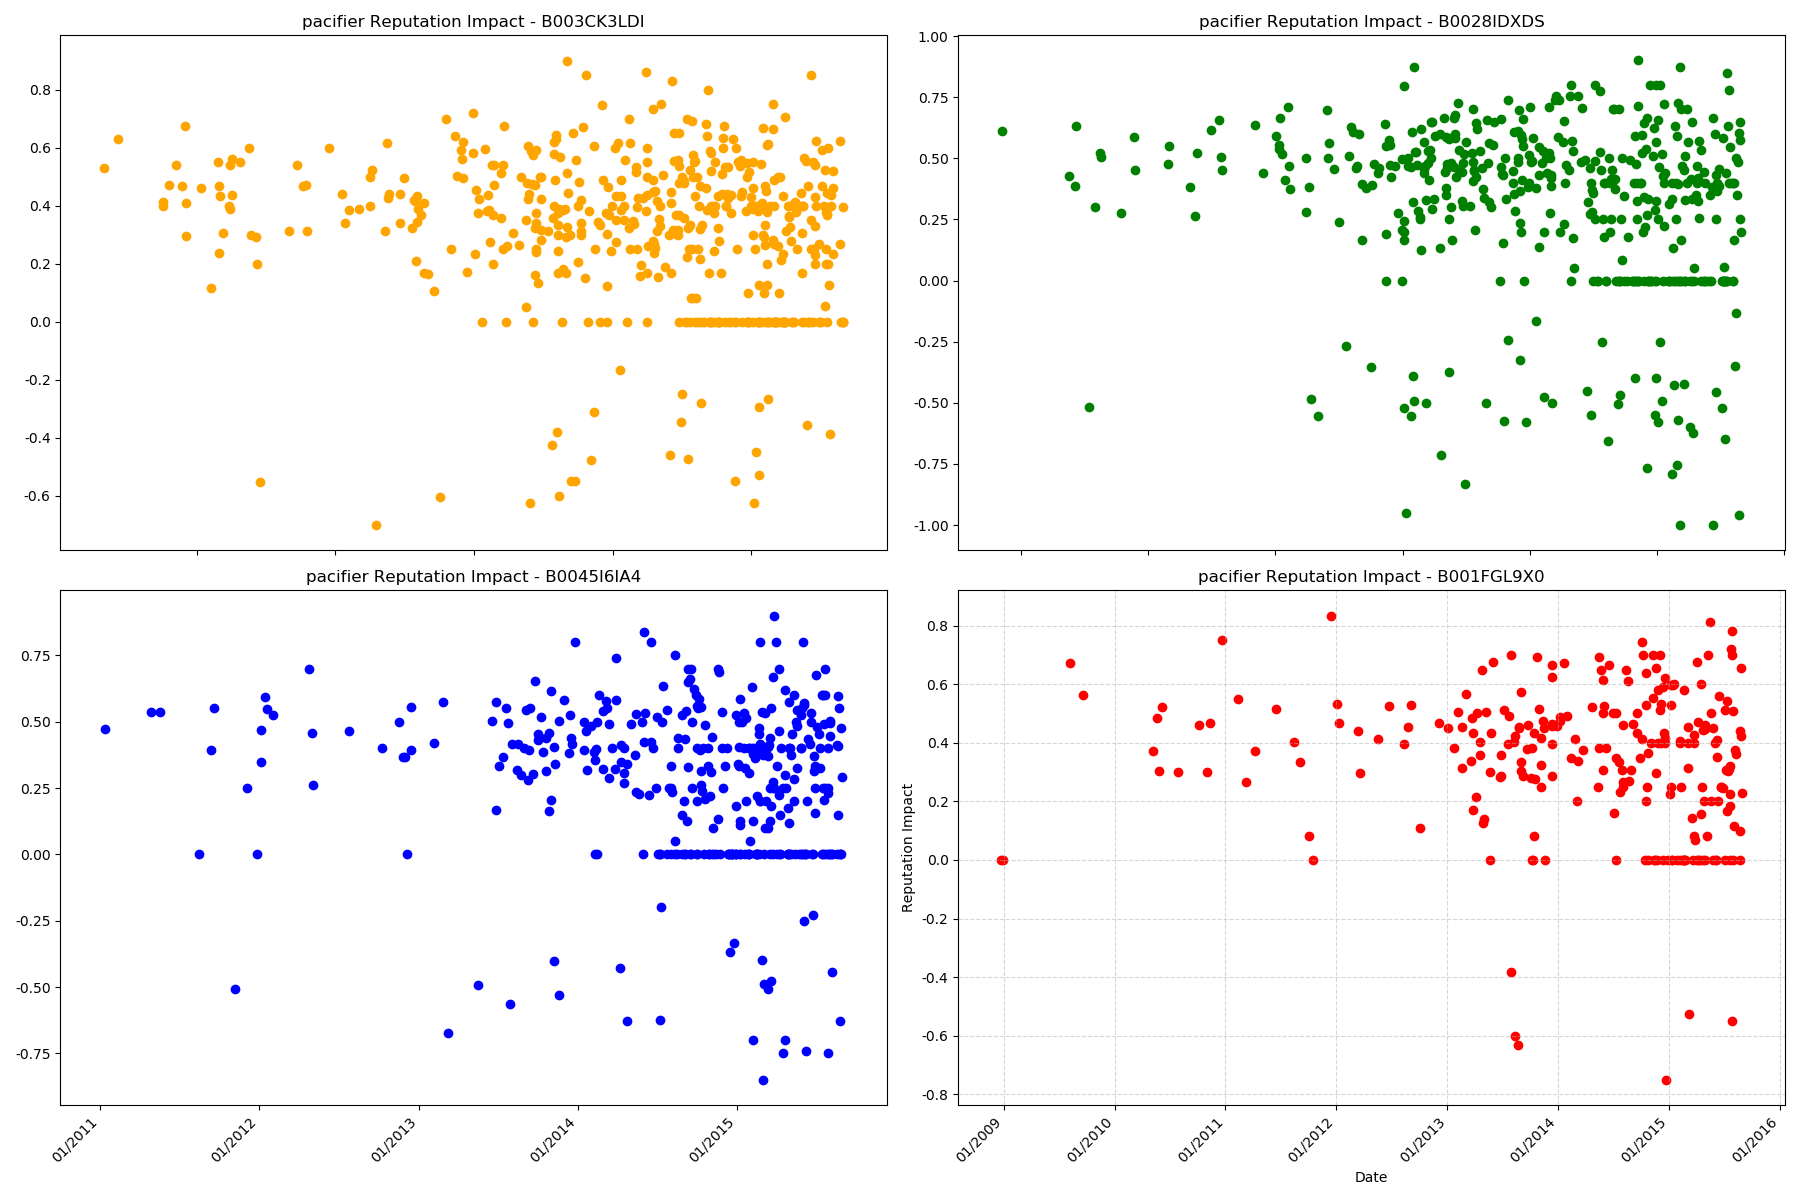
\includegraphics[width=7cm]{./figures/q2p1p.png}
	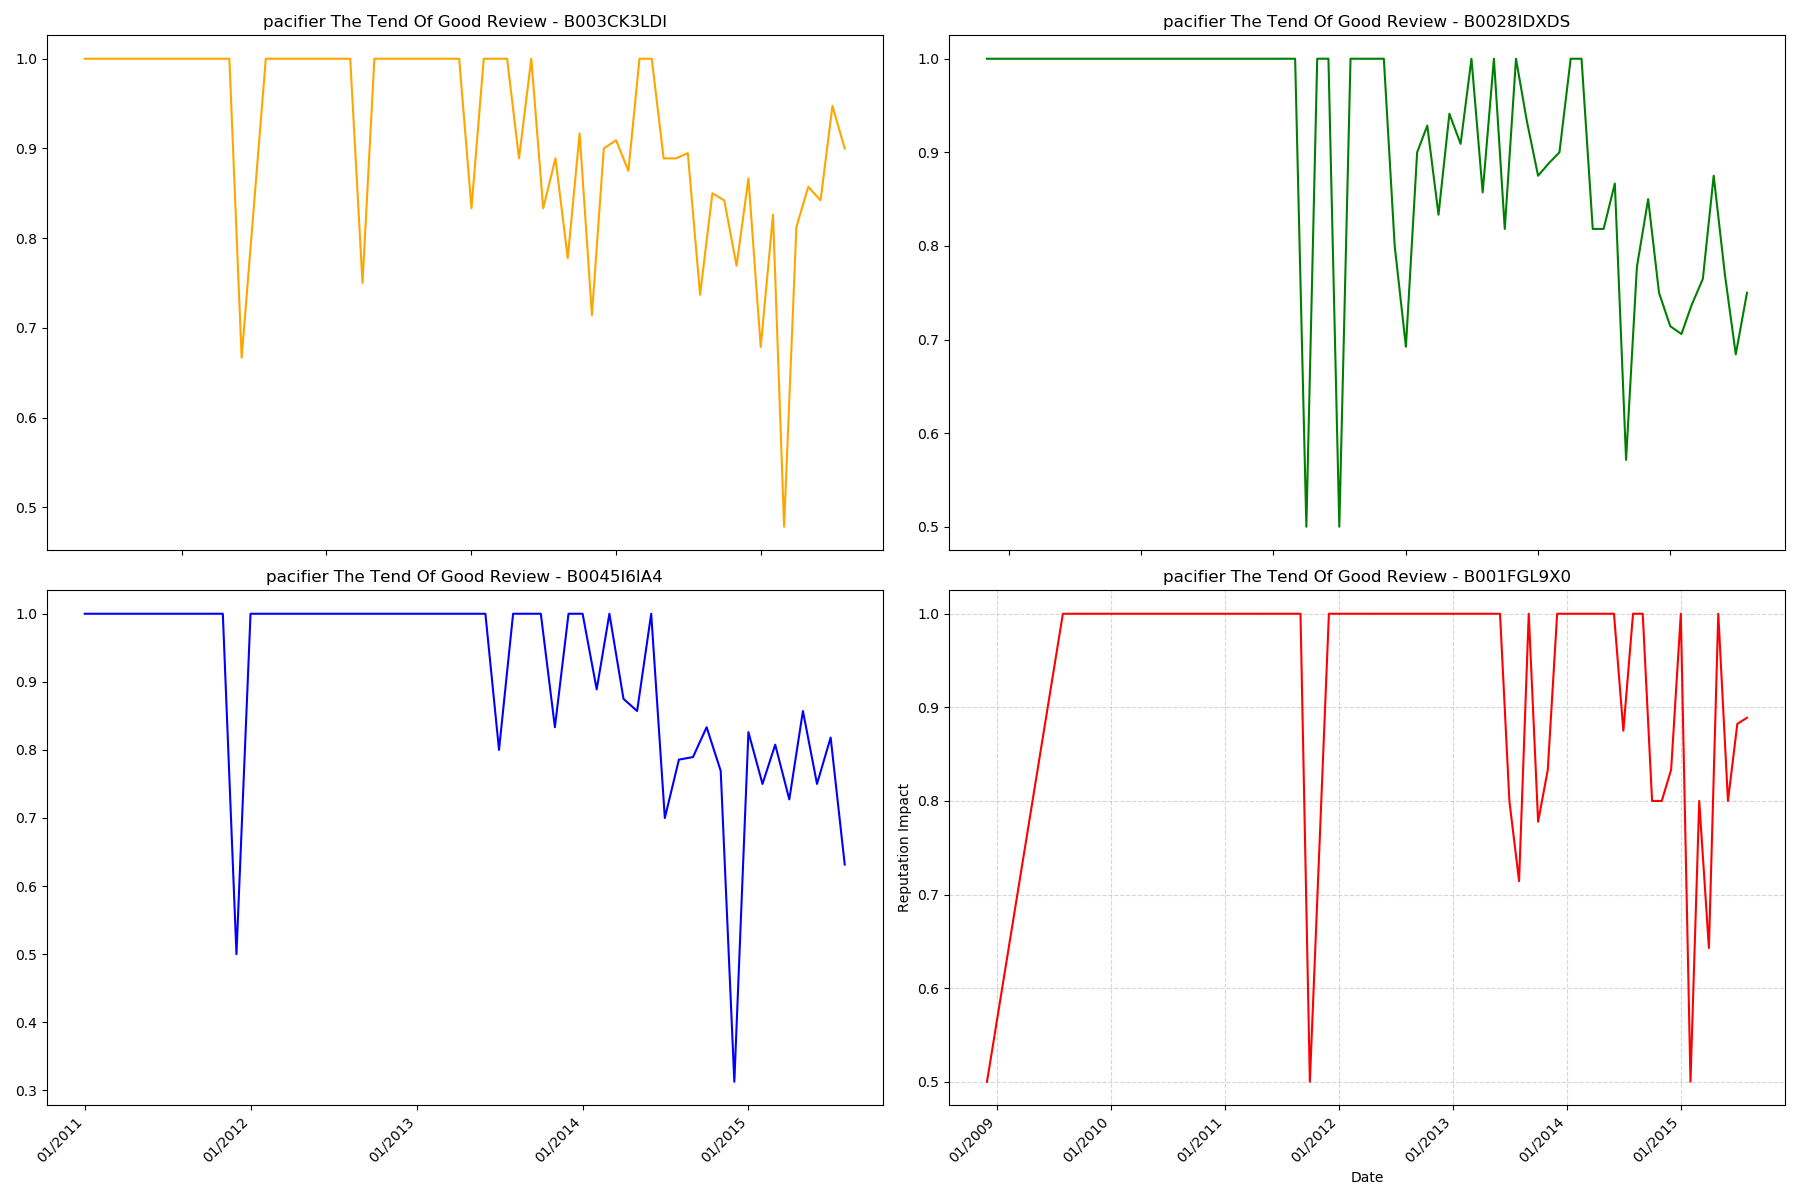
\includegraphics[width=7cm]{./figures/q2p2p.png}
	\caption{Left: reputation score of each reviewer of the top four products reviewed in the baby pacifier data; Right: monthly reputation scores for the top four products reviewed in the baby pacifier data} \label{q2p1}
\end{figure}

Figure \ref{q2p1} shows that the reputation scores of the top four products with the number of comments are mostly concentrated above 0, which indicates that most people have positive comments on the products (the same conclusion as the figure \ref{z1_q1p1} on the right). Here we are looking at the top four products in terms of the number of reviews, so these products also have high sales.

Figure \ref{q2p1} the right graph studies the proportion of the number of five-star comments to the total number of comments in a month. Reputation scores are stable at 0.5 or above, and the occasional five-star review for the month is good for the sales company. Around 2015, reputation took a turn for the worse and then stabilized. As online shopping becomes more and more common and the review data keeps increasing, it is not possible to display every comment on the shopping platform, so the network companies make corresponding adjustments to the display of comments on the shopping platform.

To sum up, sales and reputation are closely related, we strongly suggest that the sunshine company should pay attention to the reputation of products.

\subsection{The Future Trend of the Product }

How do we define success after a product has been sold in an online marketplace? If the product has been bought by many people, the comments after purchase are mostly positive, and the product has a good reputation on the Internet, then the future trend of the product must be good.

\begin{figure}[H]
	\centering
	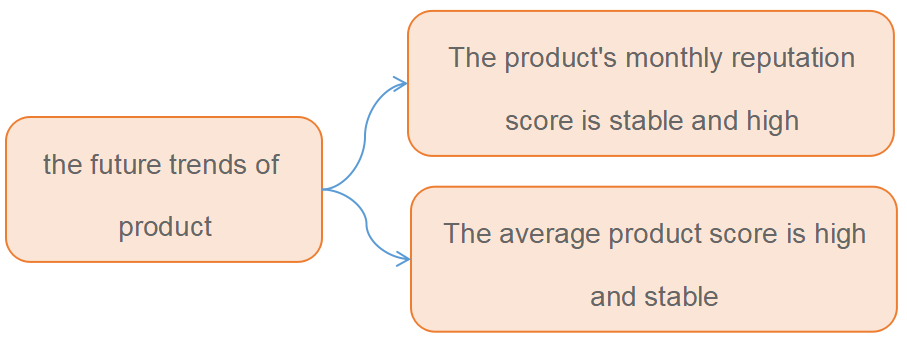
\includegraphics[width=7cm]{./figures/q3p1.png}
	\caption{the combination to indicate a potentially successful or failing product.} \label{q3p11}
\end{figure}

Reputation score and product score are important factors affecting the future development of a product. According to the formula \ref{zy1}, it can be known that the product score $f3_i$is a comprehensive indicator to measure the product quality. According to the formula \ref{gs1}, we can know that the reputation score will affect the future sales of the product. These two indicators, one to measure the quality of product attributes, the other reflects the social value, together they can have a comprehensive forecast of the future trend of the product. Product future development score $\psi$:

\begin{equation}\label{gs4q1}
\psi_j=\mathbf{avg}\sum (f_{2jk}+rp_{jk})
\end{equation}

\begin{table}[H]	
	\caption{Comparison of three indicators for different products}\label{biao4q1}
	\centering
	\begin{tabular}{c|cccc}
		\hline &review number & product score  & product reputation  & total  \\
		product id &$n_j$ & $f_{2j}$ & $rp_{j}$ & $\psi_j$ \\
		\hline B0009XH6TG & 555 & 53.76 & 13.30 & 67.06 \\
		B00VRN7SB8 & 15 & 3.37 & 16.00 & 19.37 \\
		B005GSZB9Q & 78 & 13.53 & 15.42 & 28.95 \\
		B00NXRHIO8 & 13 & 4.57 & 17.62 & 22.18 \\
		B003CK3LDI & 515 & 54.13 & 13.04 & 67.17 \\
		B00UH2XBOS & 14 & 2.65 & 13.31 & 15.96 \\
		\hline
	\end{tabular}
\end{table}

From the table \ref{biao4q1}: the more reviews the product has, the higher the future development score. Because the more reviews a product sells, the more reviews there are, the more reviews there are, so the number of reviews indirectly represents the number of sales. If we can prove that the number of comments is positively correlated with the score of future development, then it can be shown that the higher the score of $\psi_j$in future development, the more sales will be generated and the more successful the product is likely to be.


\section{Modifications of our model}%模型改进


\section{Sensitivity Analysis}


\section{Strengths and Weaknesses}



\subsection{Strengths}
\begin{itemize}
	\item 
	
	\item
	
	\item
	
	\item
	
\end{itemize}

\subsection{Weaknesses}
\begin{itemize}
	\item 
	
	\item
	
	\item
	
	\item
	
\end{itemize}

\addcontentsline{toc}{section}{Reference}
%\nocite{Bibtexkey}
\bibliographystyle{plain}
\bibliography{myreference}


\end{document}
%%
%% This work consists of these files mcmthesis.dtx,
%%                                   figures/ and
%%                                   code/,
%% and the derived files             mcmthesis.cls,
%%                                   mcmthesis-demo.tex,
%%                                   README,
%%                                   LICENSE,
%%                                   mcmthesis.pdf and
%%                                   mcmthesis-demo.pdf.
%%
%% End of file `mcmthesis-demo.tex'.

